%% This is file `elsarticle-template-1-num.tex',
%%
%% Copyright 2009 Elsevier Ltd
%%
%% This file is part of the 'Elsarticle Bundle'.
%% ---------------------------------------------
%%
%% It may be distributed under the conditions of the LaTeX Project Public
%% License, either version 1.2 of this license or (at your option) any
%% later version.  The latest version of this license is in
%%    http://www.latex-project.org/lppl.txt
%% and version 1.2 or later is part of all distributions of LaTeX
%% version 1999/12/01 or later.
%%
%% Template article for Elsevier's document class `elsarticle'
%% with numbered style bibliographic references
%%
%% $Id: elsarticle-template-1-num.tex 149 2009-10-08 05:01:15Z rishi $
%% $URL: http://lenova.river-valley.com/svn/elsbst/trunk/elsarticle-template-1-num.tex $
%%
\documentclass[preprint,12pt]{elsarticle}

%% Use the option review to obtain double line spacing
%% \documentclass[preprint,review,12pt]{elsarticle}

%% Use the options 1p,twocolumn; 3p; 3p,twocolumn; 5p; or 5p,twocolumn
%% for a journal layout:
%% \documentclass[final,1p,times]{elsarticle}
%% \documentclass[final,1p,times,twocolumn]{elsarticle}
%% \documentclass[final,3p,times]{elsarticle}
%% \documentclass[final,3p,times,twocolumn]{elsarticle}
%% \documentclass[final,5p,times]{elsarticle}
%% \documentclass[final,5p,times,twocolumn]{elsarticle}

%% The graphicx package provides the includegraphics command.
\usepackage{graphicx}
%% The amssymb package provides various useful mathematical symbols
\usepackage{amssymb}
\usepackage{amsmath}
%% The amsthm package provides extended theorem environments
%% \usepackage{amsthm}
\usepackage[version=4]{mhchem}
\usepackage{hyperref}
\usepackage{color}

%% The lineno packages adds line numbers. Start line numbering with
%% \begin{linenumbers}, end it with \end{linenumbers}. Or switch it on
%% for the whole article with \linenumbers after \end{frontmatter}.
\usepackage{lineno}

%% natbib.sty is loaded by default. However, natbib options can be
%% provided with \biboptions{...} command. Following options are
%% valid:

%%   round  -  round parentheses are used (default)
%%   square -  square brackets are used   [option]
%%   curly  -  curly braces are used      {option}
%%   angle  -  angle brackets are used    <option>
%%   semicolon  -  multiple citations separated by semi-colon
%%   colon  - same as semicolon, an earlier confusion
%%   comma  -  separated by comma
%%   numbers-  selects numerical citations
%%   super  -  numerical citations as superscripts
%%   sort   -  sorts multiple citations according to order in ref. list
%%   sort&compress   -  like sort, but also compresses numerical citations
%%   compress - compresses without sorting
%%
%% \biboptions{comma,round}

% \biboptions{}

\journal{Geochimica et Cosmochimica Acta}

\begin{document}

\begin{frontmatter}

%% Title, authors and addresses

\title{Notes on the creation and manipulation of solid solution models}

%% use the tnoteref command within \title for footnotes;
%% use the tnotetext command for the associated footnote;
%% use the fnref command within \author or \address for footnotes;
%% use the fntext command for the associated footnote;
%% use the corref command within \author for corresponding author footnotes;
%% use the cortext command for the associated footnote;
%% use the ead command for the email address,
%% and the form \ead[url] for the home page:
%%
%% \title{Title\tnoteref{label1}}
%% \tnotetext[label1]{}
%% \author{Name\corref{cor1}\fnref{label2}}
%% \ead{email address}
%% \ead[url]{home page}
%% \fntext[label2]{}
%% \cortext[cor1]{}
%% \address{Address\fnref{label3}}
%% \fntext[label3]{}


%% use optional labels to link authors explicitly to addresses:
%% \author[label1,label2]{<author name>}
%% \address[label1]{<address>}
%% \address[label2]{<address>}

\author[bristol]{Bob Myhill}
\address[bristol]{School of Earth Sciences, University of Bristol}
\cortext[mycorrespondingauthor]{Corresponding author: R. Myhill}
\ead{bob.myhill@bristol.ac.uk}


\author[ethz]{Jamie Connolly}
\address[ethz]{Institut f\"{u}r Mineralogie und Petrographie ETH-Zentrum, Claussiusstrasse 25. CH-8092, Z\"{u}rich, Switzerland}

\begin{abstract}
% Mathematical/geometrical definition of solid solutions
A large class of solid solution models start from the premise that exchange of chemical species takes place on a finite number of unique sites, and that the thermodynamic properties of the solution at any given temperature are a function of the proportions of species occupying each of the sites. The site-occupancy space spanned by such models is geometrically equivalent to a convex polytope, the $n$-dimensional equivalent of a polyhedron, where the endmembers of the solution correspond to the vertices of the polytope.

We present a set of mathematical tools based on this geometrical equivalence which aid the creation and manipulation of solution models. Vertex enumeration methods can be used to compute the total set of endmembers in a solution from the valences(?) of the species occupying each site and the total charge of the species not involved in site exchange. The number of independent endmembers constructed in this way is equal to $n_{\textit{site-species}} - n_{\textit{sites}} + c$, where $n_{\textit{site-species}}$ is the total number of potential site-species occupancies in the solution and $n_{\textit{sites}}$ is the number of distinct sites. If charge-balance constraints are active, $c=0$, otherwise $c=1$. The site-occupancy space of models able to undergo isochemical ordering may contain regions which are never energetically stable, potentially reducing the number of independent endmembers required to model the system.

% Solution model parameterisation, change of basis
We also present the linear algebra required to transform several solution model parameterisations between different independent endmember bases, and show that the same algebra can be used to calculate macroscopic endmember interactions from microscopic site interactions. This is useful both for the initial design of solution models, and for thermodynamic calculations in restricted chemical subsystems.

% Implementation
The algorithms described here are implemented in the open-source software \emph{burnman}.
\end{abstract}

\begin{keyword}
solid \sep solution \sep reciprocal \sep creation \sep manipulation
%% keywords here, in the form: keyword \sep keyword

%% MSC codes here, in the form: \MSC code \sep code
%% or \MSC[2008] code \sep code (2000 is the default)

\end{keyword}

\end{frontmatter}

%%
%% Start line numbering here if you want
%%
\linenumbers

%% main text
\section{Introduction}
\label{sec:introduction}
% Introduction

% Motivation
 Solid solution models are an essential component in modelling geological, metallurgical and other chemical processes. There are two main classes of solid solutions: substitutional, where different species substitute for each other on one or more distinct sites within the crystal lattice (for example, magnesium and iron on octahedral sites in olivine), and interstitial, where species can fill holes in the crystal structure (for example, carbon in steel). [the importance of this distinction is not evident to me, isn't interstitial just substitution of an ion for a vacancy?]

The motivation behind this paper is to introduce some mathematical background defining the structure and properties of commonly used substitutional [i.e., the paper is inapplicable to interstitial models?] solution models, and to introduce tools that aid in their construction and manipulation. We concentrate on solution models which have a constant number of sites per formula unit, and where interactions are dependant only on the total proportions of species occupying each site. We do not consider models which explicitly involve local interactions, such as bonding between pairs or clusters of species \citep[e.g.][]{Bethe1935,Inden2001}.

\section{An algebraic description of solid solutions}
\subsection{Solid solutions as polytopes}
\label{sec:polytope_description}
Substitutional solid solutions can be written in the form:
\begin{equation}
    \ce{[A, B]^Y_y[B, C, D]^Z_z}...
    \label{eqn:soln}
\end{equation}
where the square brackets denote distinct sites in the structure, and the comma-separated lists are the species that can occupy each site. In the example above, species A and B can occupy Site Y, which has a multiplicity of $y$ in the formula unit, and species B, C and D can occupy Site Z, which has a multiplicity of $z$. Throughout this paper, the species which can occupancy each site for any given solution are called \emph{site-species}. There are five site-species in Equation \ref{eqn:soln} (\ce{A^Y}, \ce{B^Y}, \ce{B^Z}, \ce{C^Z}, \ce{D^Z}, ; $n_{\textit{site-species}} = 5$).

We define the site-occupancy space of any solid solution as the set of site-species occupancies on sites which satisfy the chemical formula of the solution. This space is mathematically equivalent to a convex polytope (the $n$-dimensional equivalent of a polyhedron). That is, the set $\mathcal{X}$ of valid site-species occupancies $\boldsymbol{x}$ of a solid solution can be described using an $m$ x $n_{\textit{site-species}}$ matrix $\boldsymbol{P}$ and a vector $\boldsymbol{b}$ of length $m$:
\begin{equation}
  \mathcal{X} = \{\boldsymbol{x}; \boldsymbol{P}\boldsymbol{x} = \boldsymbol{b}; x \ge 0 \}
  \label{eqn:polytope_set}
\end{equation}
where m is the number of independent constraints on the site populations (?).
For single-site solution models with $k$ endmembers, the matrix $\boldsymbol{P}$ is simply a 1x$k$ vector of ones, and $b$=1, such that the requirements for the solution can be rewritten as
\begin{equation}
  \sum_{i=1}^{k} x_i = 1
\end{equation}
Such polytopes are $(k-1)$-simplexes, the $(k-1)$-dimensional equivalent of a triangle. For multi-site solution models where each site can be occupied only by species with equal charges, matrix $\boldsymbol{P}$ has $n_{\textrm{sites}}$ rows. Each row corresponds to a distinct site (such as the dodecahedral site in garnet), and each column to a potential elemental occupancy (such as Mg on the dodecahedral site). The components of the matrix are equal to zero unless the column and row correspond to the same site, in which case the components are equal to one. Non-simplicial polytopes are the cartesian product of the $n_{\textrm{sites}}$ site-simplices.

Charge-balance can be incorporated as an additional row in matrix $\boldsymbol{P}$ and component in vector $\boldsymbol{b}$, with the new components of $\boldsymbol{P}$ corresponding to the charges of each site-species multiplied by the site multiplicity, and the new value in $\boldsymbol{b}$ corresponding to the total charge over all the sites. This additional row represents a hyperplane cutting through the original polytope. Graphical representations of 1-, 2- and 3-site solution model polytopes, with and without charge-balance constraints are shown in Figure \ref{fig:solution_polytopes}. 

\begin{figure}[htb!]
  \centering
  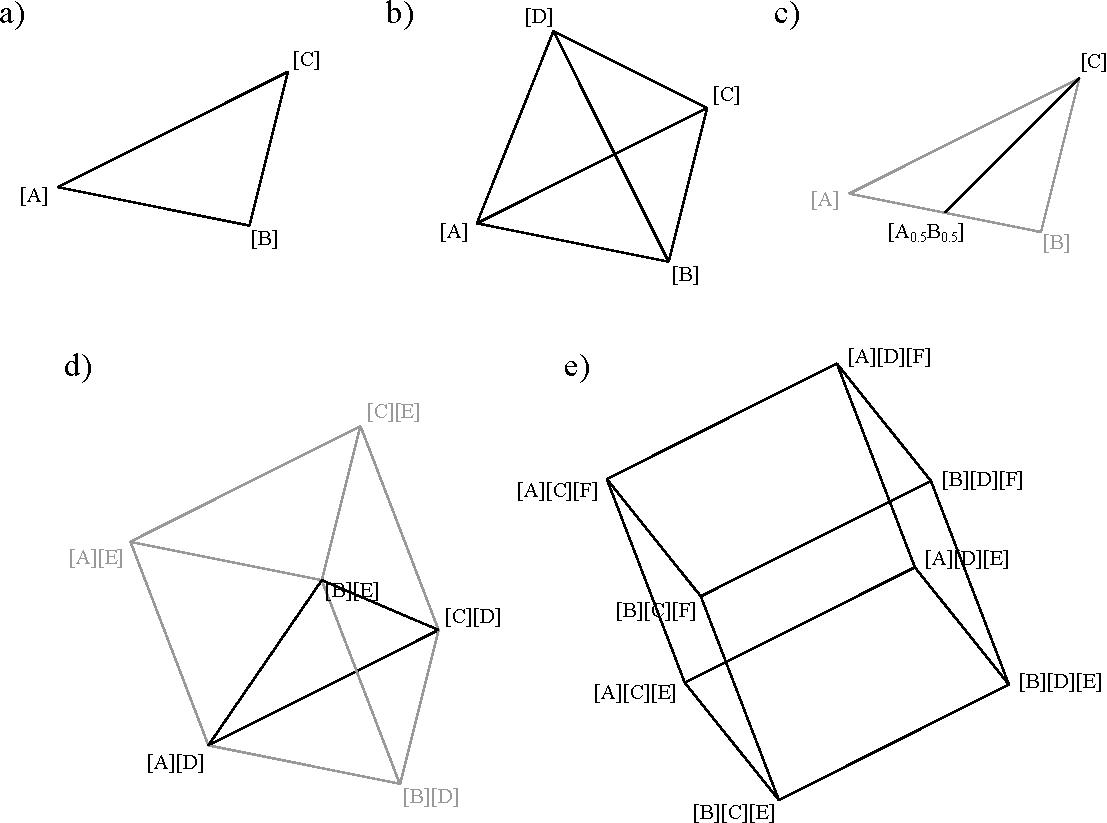
\includegraphics[width=\textwidth]{figures/solid_solution_polytopes.pdf}
  \caption{Polytopes corresponding to some 1-site (a-c), 2-site (d) and 3-site (e) solution models. The dimensionality of an $n$-site solution model without charge-balance constraints is equal to $\sum_{i=1}^n (k_i - 1)$, where $k_i$ is the number of endmembers on site $i$, restricting the variety of polytopes which can be represented graphically in 3-dimensions. a) A 2-simplex, such as \ce{[Mg,Fe,Ca]3Al2Si3O12} garnet. b) A 3-simplex, such as \ce{[Mg,Fe,Ca,Mn]3Al2Si3O12} garnet. c) A subset of a 2-simplex, such as a one-site pyrope-majorite solution \ce{Mg3[Mg,Al,Si]2Si3O12}, where a charge-balance constraint limits the valid site-occupancy space (see Table \ref{tab:maj_polytope}). Grey lines mark the original 2-simplex without charge-balance constraints. d) A subset of the cartesian product of a 3-simplex and 2-simplex, such as \ce{[Fe,Mg,Al][Al,Si]O3}-bridgmanite (Table \ref{tab:bdg_polytope}). Grey lines mark the original polytope without charge-balance constraints. e) The cartesian product of three 2-simplexes, e.g. \ce{[Cu,Ag]10[Fe,Zn]2[Sb,As]4S13} fahlore \citep{Sack2017}.}
  \label{fig:solution_polytopes}
\end{figure}

Let us look at two examples, bridgmanite and majorite, in detail. Table \ref{tab:bdg_polytope} shows the matrix $\boldsymbol{P}$ and vector $\boldsymbol{b}$ for a two-site bridgmanite in the system \ce{FeO-MgO-Al2O3-SiO2}, which in the form given in Equation \ref{eqn:soln} can be expressed as 
\begin{equation*}
\ce{[Fe^{2+}, Mg^{2+}, Al^{3+}][Al^{3+}, Si^{4+}]O3}.
\end{equation*}

\begin{table}[htb!]
\centering
\begin{tabular}{llllll|l}
               & \multicolumn{3}{l}{Site A}      & \multicolumn{2}{l}{Site B} &   \\
               & Fe$^{2+}$ & Mg$^{2+}$ & Al$^{3+}$ & Al$^{3+}$ & Si$^{4+}$ & b \\
               \hline
A-site         & 1    & 1    & 1    & 0    & 0    & 1 \\
B-site         & 0    & 0    & 0    & 1    & 1    & 1 \\
Charge-balance & 2    & 2    & 3    & 3    & 4    & 6
\end{tabular}
\caption{Polytope matrix $\boldsymbol{P}$ and vector $\boldsymbol{b}$ for a two-site FMAS bridgmanite including full order-disorder.}
\label{tab:bdg_polytope}
\end{table}

The vertices of the polytope which satisfies Equation \ref{eqn:polytope_set} have components of $x$ equal to either 0 or 1 \{[0,1,0,0,1], [1,0,0,0,1], [0,0,1,1,0]\}, and thus correspond to a subset of the six vertices of the polytope formed without the charge-balance constraint. This polytope is represented graphically in Figure \ref{fig:solution_polytopes}d. Each vertex corresponds to an ordered endmember in the solid solution (where here we use the word order to mean that only one element occupies each site) \{[Mg][Si], [Fe][Si], [Al][Al]\}.[mentioning the difference with H&P usage might be worthwhile, i.e., an ordered endmember is a fully ordered endmember that includes at least two chemically distinct disorderable site-species and anything else is a "disordered" endmember]

Some solutions have disordered endmembers (where one or more sites contain multiple elements). for example, pyrope-majorite garnet. At extremely high temperatures [ref?], this solution can be treated by considering mixing on a single octahedral site (\ce{Mg3[Mg,Al,Si]2Si3O12}). Table \ref{tab:maj_polytope} provides the corresponding polytope matrix and vector.
\begin{table}[htb!]
\centering
\begin{tabular}{llll|l}
               & \multicolumn{3}{l}{Site Y (multiplicity 2)} &   \\
               & Mg$^{2+}$ & Al$^{3+}$ & Si$^{4+}$ & b \\
               \hline
Y-site         & 1    & 1    & 1    & 1 \\
Charge-balance & 4    & 6    & 8    & 12
\end{tabular}
\caption{Polytope matrix $\boldsymbol{P}$ and vector $\boldsymbol{b}$ for a one-site pyrope-majorite garnet.}
\label{tab:maj_polytope}
\end{table}
This polytope is equivalent to that plotted in Figure \ref{fig:solution_polytopes}c, with the two vertices corresponding to pyrope (\ce{Mg3[Al]2Si3O12}) and disordered majorite (\ce{Mg3[Mg_{0.5}Si_{0.5}]2Si3O12}). At the more moderate temperatures characteristic of the mantle, pyrope-majorite garnets are better described by a model with two distinct octahedral sites (Table \ref{tab:maj2_polytope}).
\begin{table}[htb!]
\centering
\begin{tabular}{lllllll|l}
               & \multicolumn{3}{l}{Site Y$_1$ (multiplicity 1)} & \multicolumn{3}{l}{Site Y$_2$ (multiplicity 1)} &   \\
               & Mg$^{2+}$ & Al$^{3+}$ & Si$^{4+}$ & Mg$^{2+}$ & Al$^{3+}$ & Si$^{4+}$ & b \\
               \hline
Y$_1$-site         & 1    & 1    & 1    & 0    & 0    & 0    & 1 \\
Y$_2$-site         & 0    & 0    & 0    & 1    & 1    & 1    & 1 \\
Charge-balance     & 2    & 3    & 4    & 2    & 3    & 4   & 12
\end{tabular}
\caption{Polytope matrix $\boldsymbol{P}$ and vector $\boldsymbol{b}$ for a two-site pyrope-majorite garnet.}
\label{tab:maj2_polytope}
\end{table}
The site-occupancy space of this model is a polytope with five endmember vertices, of which any four are linearly independent. A possible set of independent endmembers is \{[Mg][Si], [Si][Mg], [Al][Al], [Al][Mg$_{0.5}$Si$_{0.5}$]\}, with the dependent endmember in this case being [Mg$_{0.5}$Si$_{0.5}$][Al]. Importantly, splitting the sites has not removed all disordered endmembers, but Mg and Si are now able to reside on separate sites. Even this model is not sufficient to describe the results of atomistic simulations at low temperatures ($<$1473 K), which predict ordering in the middle of the pyrope-majorite binary join \citep{Vinograd2006}. A four-site model with eight independent endmembers is required to reproduce(?) this behaviour (see Section \ref{sec:sro}). 

\subsection{Endmember enumeration}
% Finding all the possible endmembers of a given solution
There are a wide range of different algorithms that can find all the vertices of a polytope given a set of equalities \citep[the ``vertex enumeration problem''; e.g.][]{MR1980,AF1992,Lasserre2004}. Vertex enumeration on the site-occupancy space of a solution model yields an endmember site-occupancy matrix $\boldsymbol{E}$, where each component $E_{ij}$ comprises the fractional occupancy of site-species $j$ in a distinct endmember $i$. 
The resulting number of vertices may be much larger than the number of site-species. For solid solutions with no charge-balance constraints, the number of endmember vertices grows geometrically with the number of sites:
\begin{equation}
    n_{\textit{mbrs}} = \prod_{i=1}^{n_{\textit{sites}}} k_i
\end{equation}
Despite the geometric growth in the \textbf{total} number of endmembers, the number of \textbf{independent} endmembers grows linearly. A potential set of independent endmembers can be computed in several ways, including as a by-product of finding the row-reduced en-echelon form of $\boldsymbol{E}$ (one such implementation is found in the algorithms described in the Appendix). Taking the dot product of resulting matrix $\boldsymbol{E}^{\textit{ind}}$ with a vector of endmember proportions $\boldsymbol{p}$ yields the site-species occupancies $\boldsymbol{x}$ of a solution:
\begin{equation}
    E^{\textit{ind}}_{ji}p_j = x_i
    \label{eqn:proportions_to_sites}
\end{equation}

\subsection{Constructing a polytope from an existing set of independent endmembers}
The previous sections described how to compute a complete set of endmembers and an independent endmember basis from a set of known site-species and their valences. This is a fundamental first-step for anyone wishing to construct a solution model, and can be a time-consuming and error-prone task to compute by-hand for more complex models. The following section describes the inverse procedure; how a set of independent endmembers can be used to construct the polytope matrix $\boldsymbol{P}$ and vector $\boldsymbol{b}$.

First, we populate the independent endmember site-occupancy matrix $\boldsymbol{E}^{\textit{ind}}$. Table \ref{tab:bdg_matrix} shows the elements of $\boldsymbol{E}^{\textit{ind}}$ for the two-site bridgmanite described in the previous section.
\begin{table}[htb!]
\centering
\begin{tabular}{llllll}
               & \multicolumn{3}{l}{Site A}      & \multicolumn{2}{l}{Site B}   \\
Endmember      & Fe$^{2+}$ & Mg$^{2+}$ & Al$^{3+}$ & Al$^{3+}$ & Si$^{4+}$  \\
\hline
\ce{[Fe][Si]O3} & 1    & 0    & 0    & 0    & 1 \\
\ce{[Mg][Si]O3} & 0    & 1    & 0    & 0    & 1 \\
\ce{[Al][Al]O3} & 0    & 0    & 1    & 1    & 0
\end{tabular}
\caption{The independent endmember site-occupancy matrix $\boldsymbol{E}^{\textit{ind}}$ for a two-site FMAS bridgmanite including full order-disorder.}
\label{tab:bdg_matrix}
\end{table}
The polytope matrix $\boldsymbol{P}$ and vector $\boldsymbol{b}$ of this solution can be computed from the right nullspace (or kernel) of $\boldsymbol{E}^{\textit{ind}}$, defined as the set of site-species occupancy vectors $\boldsymbol{x}$ which satisfy the expression:
\begin{equation}
  \mathcal{N}(\boldsymbol{E}^{\textit{ind}}) = \{\boldsymbol{x}; \boldsymbol{E}^{\textit{ind}}\boldsymbol{x} = \boldsymbol{0}\}
  \label{eqn:nullspace_site_occupancy_matrix}
\end{equation}
Note that Equations \ref{eqn:nullspace_site_occupancy_matrix} and \ref{eqn:polytope_set}; both are sets based on a set of linear equalities involving the site-species occupancy vectors. Indeed, the sets can be made identical by adding to Equation \ref{eqn:nullspace_site_occupancy_matrix} the requirement that the sum of the site-species occupancy fractions equals the number of sites. Therefore, a polytope matrix $\boldsymbol{P}$ can be constructed by adding a row of ones to the right nullspace of $\boldsymbol{E}^{\textit{ind}}$, and the vector $\boldsymbol{b}$ can be constructed from the null vector $\mathbf{0}$ by appending a component with value equal to the number of sites in the solution.  
 
 This construction reveals a relationship between the shape of $\boldsymbol{E}^{\textit{ind}}$ and the number of constraints $m$ defining the polytope. As the $n_{\textit{ind-mbrs}}$ x $n_{\textit{site-species}}$ matrix $\boldsymbol{E}^{\textit{ind}}$ is, by-definition, of full row-rank, the dimension of the nullspace of $\boldsymbol{E}^{\textit{ind}}$ (its nullity) must be equal to $n_{\textit{site-species}} - n_{\textit{ind-mbrs}}$. As $\boldsymbol{P}$ can be constructed by adding a single row to $\mathcal{N}(\boldsymbol{E}^{\textit{ind}})$, it follows that
 \begin{equation}
 \begin{split}
     m &= \textrm{rank}(\boldsymbol{P}) \\
     &= \textrm{nullity}(\boldsymbol{E}^{\textit{ind}}) + 1 \\
     &= n_{\textit{site-species}} - n_{\textit{ind-mbrs}} + 1
\end{split}    
    \label{eqn:ind_mbrs}
 \end{equation}
From Section \ref{sec:polytope_description}, $m$ is equal to the number of sites, plus one if charge-balance needs to be considered. Thus, the number of independent endmembers describing a fully-consistent solid solution is governed by the relationship:
 \begin{equation}
     n_{\textit{ind-mbrs}} = n_{\textit{site-species}} - n_{\textit{sites}} + c
     \label{eqn:site_mbr_relationship}
 \end{equation}
where $c=0$ if charge-balance needs to be considered, and $c=1$ otherwise. 

\subsection{Subspaces and degeneracy within solid solutions}

The shape of the polytope defining a solid solution depends only on the number of sites, and the number and total charge of site-species on those sites. It does not depend on whether the same site-species [i would minimize the number of descriptive terms used here, already by themselves component/species are not well understood terms] (e.g. \ce{Fe^{2+}}) resides on multiple sites. Figure \ref{fig:subspaces} shows polytopes for two three-site solutions, one with different site-species [i suppose it's possible to debate whether "site" already carries a site-specific connotation, i.e., Fe on M1 is not the same "site-species" as Fe on M2, which is sort of the point you make here, but in that case i favor the term ion/cation instead of component]   on all sites ([A,B][C,D][E,F]), and one where the same [components] appear on all three sites ([A,B][A,B][A,B]).

In (a), there is no overlap among the site-species on the three sites. The shaded tetrahedron is bounded by one set of potential independent endmembers. The rest of the polytope can be constructed from linear combinations of these endmembers. Every point within the polytope has a unique composition. In (b), the three sites are instead filled with the same sets of site-species. Again, the shaded tetrahedron shows the subspace of the solution bounded by one potential set of independent endmembers. However, this time the full compositional range is spanned by a single line from endmember AAA to endmember BBB. Depending on the interactions within and between sites, there are several possibilities regarding degeneracy and how much of the total site-occupancy space may be stable:

\begin{itemize}
    \item If there is no preference for A or B to reside on any one site, all stable points will lie along AAA--BBB, i.e., the solution is fully disordered.
    \item If all three sites are identical in terms of same- and cross-site interaction energies, the tetrahedron contains all the relevant thermodynamics of the system; the distribution of excess energies will be duplicated in the five other tetrahedra. [this is unclear to me, won't the speciation again be on the aaa-bbb join?]
    \item If the three sites have different energies, one or more tetrahedra may only be stable at particular conditions, or never be stable under any circumstances. We will elaborate on this case in the next section, i.e., the solution is partially, or fully, ordered.
\end{itemize}



\begin{figure}[htb!]
  \centering
  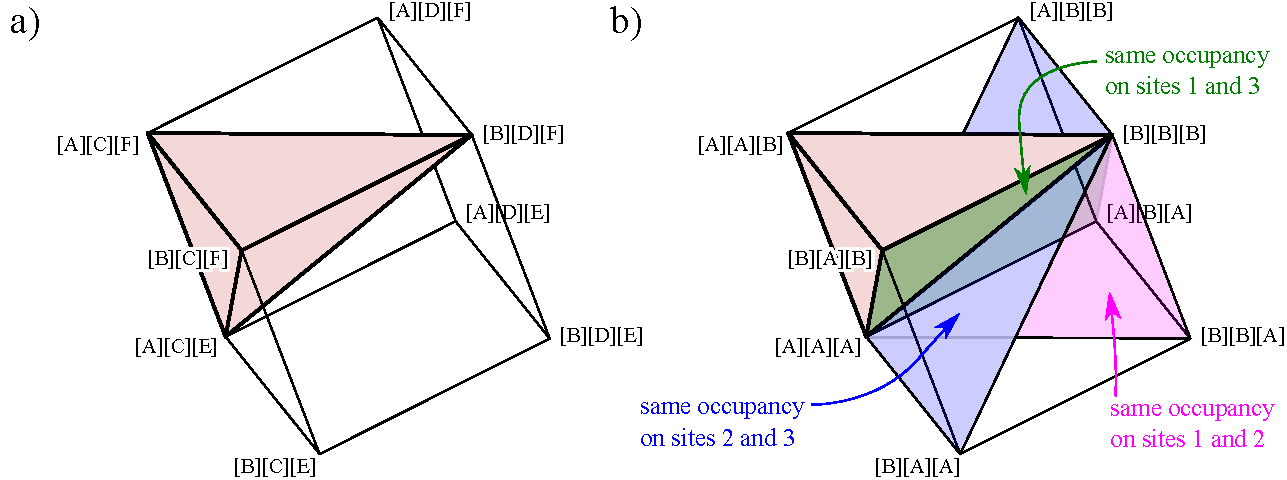
\includegraphics[width=\textwidth]{figures/solid_solution_polytopes_degenerate.pdf}
  \caption{Polytopes for two three-site solutions and a subspace bounded by a set of independent endmembers. a) The three sites are filled with different [components]: [A,B][C,D][E,F]. The shaded tetrahedron shows the subspace of the solution bounded by one potential set of independent endmembers. b) The three sites are instead filled with similar components: [A,B][A,B][A,B]. Coloured planes mark where there is complete disorder between two sites. Again, the shaded tetrahedron shows the subspace of the solution bounded by one potential set of independent endmembers. Note the tetrahedron is also bounded by the planes marking two-site disorder.}
  \label{fig:subspaces}
\end{figure}

\subsection{Unstable subspaces, metastable compounds and potential simplifications to order-disorder models}
\label{sec:relative_stability}
[this section needs some clarification of what you mean by stability, you are using the term in ways that vaguely relate to internal/homogeneous/heterogeneous equilibrium but not clearly to the 2nd law concept]
In the case of solution models where each endmember represents a different composition, each point within the site-occupancy space also represents a different composition, and is therefore stable under all conditions [this is not true in the 2nd law sense, i.e., the composition maybe metastable with respect to heterogeneous equilibrium with the same bulk composition]. In contrast, models with some compositional [it would be clearer to distinguish speciation and composition, this could be done by observing that there are two polytopes, degeneracy in the present context refers to the case that the compositional polytope has fewer dimensions than the speciation polytope] degeneracy (where ordering of atoms occurs on two or more sites) there will be parts of site-occupancy space which are unstable at any given condition [in fact, each independent order parameter removes a dimension from the speciation space]. The simplest example is two site Fe-Mg exchange (\ce{[Fe,Mg][Fe,Mg]}, where a unique (or at most two-fold degenerate) distribution of Fe and Mg will be the most stable at any given composition, pressure and temperature.

There are also cases where parts of site-occupancy space are unstable at all temperatures and pressures. Taking again the example of Fe-Mg exchange, if ordering is unstable at 0 K (not physically plausible, but certainly mathematically possible), the entire solution may be modelled using only the endmembers \ce{[Mg][Mg]} and \ce{[Fe][Fe]} [i don't see the value of this example, in fact this section doesn't add much because the paper doesn't really treat the thermodynamics of solving for the stable speciation]. A slightly more complex example is the two-site pyrope-majorite garnet discussed in Section \ref{sec:polytope_description}. At a \ce{Mg3(AlMg_{0.5}Si_{0.5})Si3O12}-composition, Al, Mg and Si may be distributed equally or unequally between the octahedral sites. The configurational entropies of binary mixing between different isochemical endmembers are shown in Figure \ref{fig:pyrope_majorite_entropy}. Of these endmembers, \ce{Mg3[Mg_{0.5}Si_{0.5}][Al]Si3O12} has the lowest configurational entropy ($R \ln 2$). If the endmember energy and interaction energies of this configuration are sufficiently high, the proportion of the endmember in the solid solution will be zero, regardless of the pressure, temperature or bulk composition of the solution.

\begin{figure}[htb!]
  \centering
  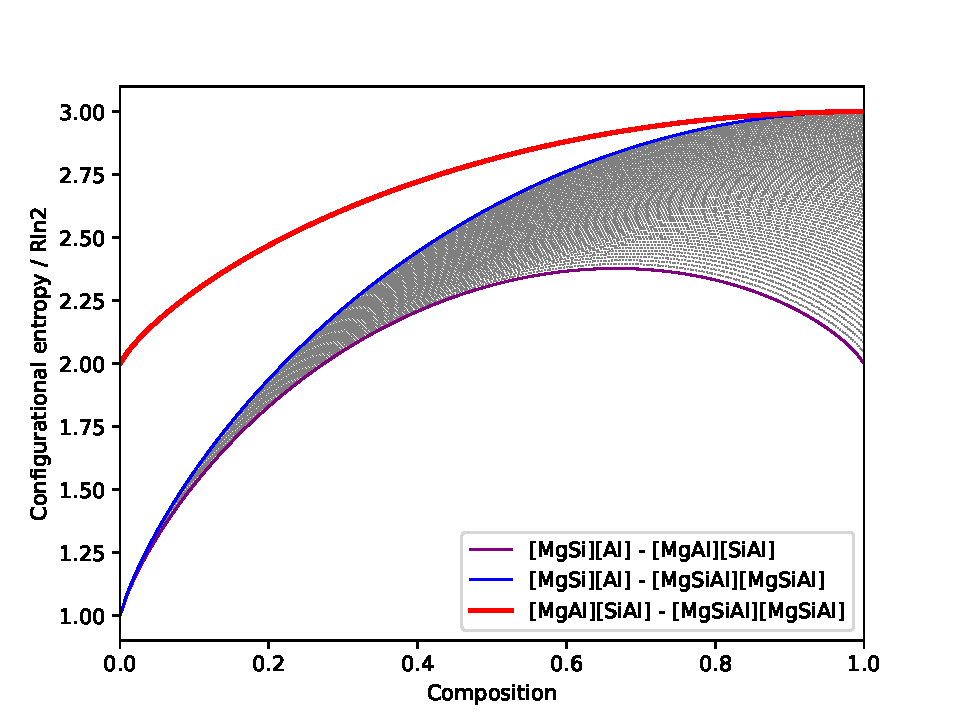
\includegraphics[width=0.80\textwidth]{figures/py_maj_entropy.pdf}
  \caption{Entropy of \ce{Mg3(AlMg_{0.5}Si_{0.5})Si3O12}-composition garnets along binary joins within the two-site pyrope-majorite solution model.}
  \label{fig:pyrope_majorite_entropy}
\end{figure}

There is ample motivation for wishing to remove endmember[the example is specific, if you want to generalize from the example, the generalization should lead or follow] \ce{Mg3[Mg_{0.5}Si_{0.5}][Al]Si3O12} from the order-disorder models/speciation polytope:
\begin{itemize}
    \item The endmember represents the lowest configurational entropy at that composition, but that entropy is non-zero. In nature, such compositions will tend to undergo further ordering (at low enough temperatures), and if ordering is observed at that composition it is generally more suitable to split the sites to allow complete ordering to take place.
    \item Moving away from the composition of the \ce{Mg3[Mg_{0.5}Si_{0.5}][Al]Si3O12} endmember requires an unlikely redistribution of elements across sites. In this case, increasing majorite content results in [Al $\leftrightarrow$ Mg][Mg $\leftrightarrow$ Si] or [Al $\leftrightarrow$ Si][Si $\leftrightarrow$ Mg]. 
    \item If the [Al][MgSi] configuration is stable at low temperatures, it will be destabilised relative to [MgAl][SiAl] as alumina content decreases and/or temperatures increase. Under these circumstances, a major redistribution of elements can take place over very small compositional and/or temperature intervals (see Figure \ref{fig:pyrope_majorite_configurations} [x-axis needs a better label]). 
    \item From a computational perspective, reducing the number of order-disorder parameters decreases the time required to find the equilibrium site distributions.
\end{itemize}

\begin{figure}[htb!]
  \centering
  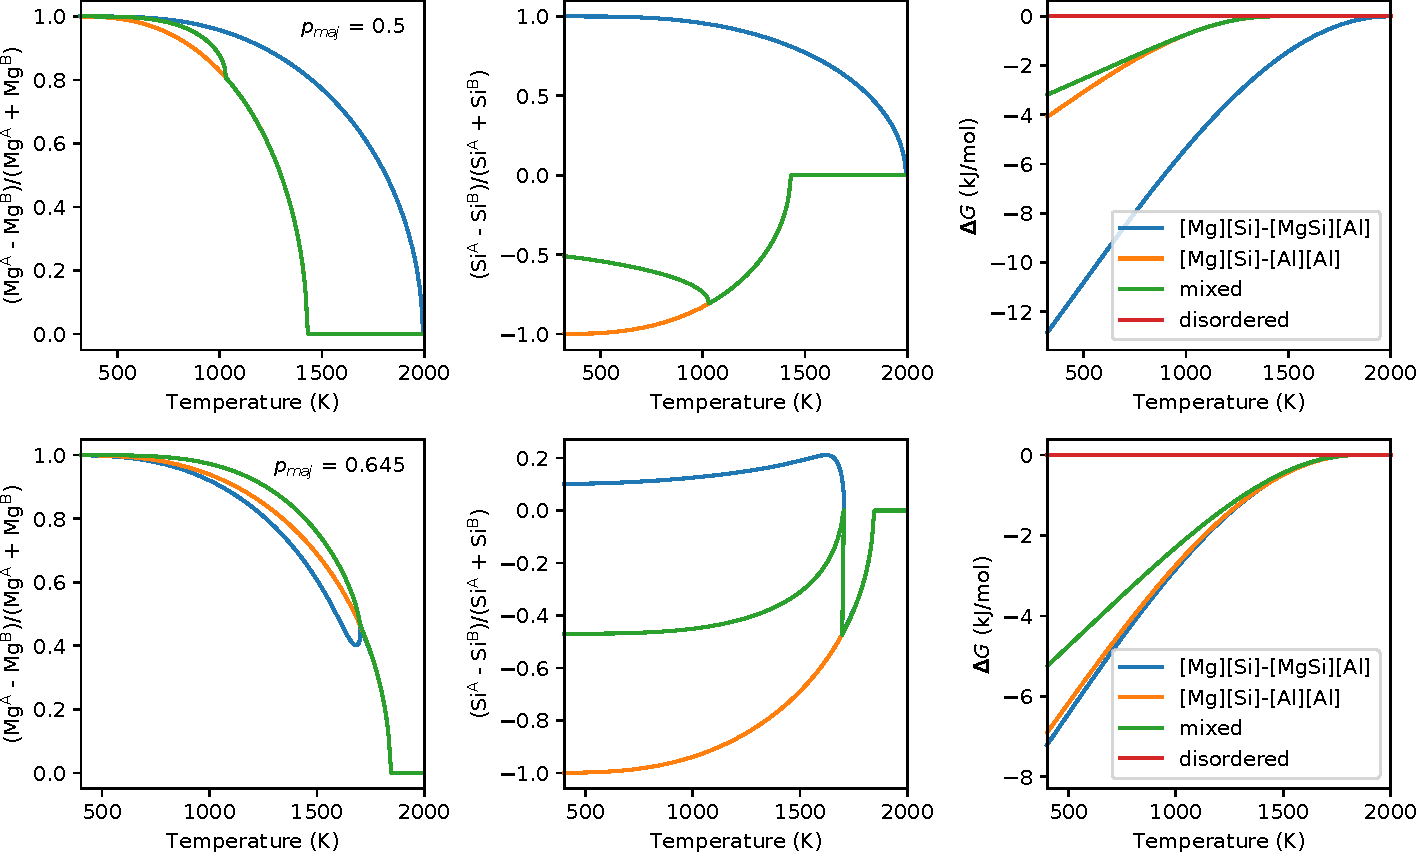
\includegraphics[width=\textwidth]{figures/py_maj_configurations_edited2.pdf}
  \caption{Stable and metastable configurations of 2-site magnesium aluminosilicate garnets having majorite-pyrope ratios of 50:50 (a--c) and 64.5:35.5 (d--f). At low temperatures, the three different configurations are dominated by mixing between [Mg][Si]--[MgSi][Al], [Mg][Si]--[Al][Al], or a mixture of [Mg][Si]--[MgSi][Al]-[Al][Al] endmembers. The relative difference in Mg and Si occupancy between the two sites are given in (a,d) and (b,e). The molar Gibbs free energy relative to that of the completely disordered compound is given in (c,f) [? DG = -T DS?]. Note the rapid change in composition at $\sim$1700 K for the stable majorite-rich garnet (blue line in e). The [MgSi][Al] endmember is destabilised for compositions with $>$65\% majorite.[a-f not indicated on figure] }
  \label{fig:pyrope_majorite_configurations}
\end{figure}

Before removing an endmember from a solution model, it is vital to check that the removal does not result in any logical inconsistencies or unexpected behaviour (see Section \ref{sec:inconsistency}). Conversely, if one is constructing a macroscopic solution model from microscopic interaction parameters (Section \ref{sec:micro_to_macro}), it may be useful to check if the parameters used allow the use of a reduced number of independent endmembers.

\subsection{Approximating short-range order}
\label{sec:sro}
Short-range ordering in solid solutions arises from local interactions within 3D lattices. The probability of a certain species residing on any given site in a lattice depends not only on the proportion of that species in the crystal, but also on the arrangement of all of the species surrounding it, because each bond with a neighbouring atom will contribute to the total internal energy \citep[e.g.][]{Bethe1935}. A first-principles consideration of these local interactions is not possible within the models considered in this paper, because the total energy of these solid solution models depends only on proportions of species averaged over all sites. However, given how rapidly model complexity increases when considering local bonding in multicomponent systems \citep[e.g.][]{Inden2001}, it is worthwhile considering whether short-range order can be reasonably approximated within these models.

% Fake site multiplicities 
% opx example
A popular method of approximating short-range order in these models is to reduce the effective number of sites on which mixing takes place. For example, \citet{SLB2011} consider the following potential enstatite--Mg-Tschermaks endmembers in orthopyroxene:
\begin{itemize}
\item \ce{Mg[Mg][Si]SiO6 - Mg[Al][Al]SiO6}
\item \ce{Mg[Mg]Si2O6 - Mg[Al]AlSiO6} (favoured)
\item \ce{[Mg]2Si2O6 - [Mg_{0.5}Al_{0.5}]2AlSiO6}
\item \ce{Mg[Mg][Si]2O6 - Mg[Al][Al_{0.5}Si_{0.5}]2O6}
\end{itemize}
As in the rest of this manuscript, square brackets denote distinct sites on which mixing takes place. All of these binaries describe the same species exchange (MgSi $\leftrightarrow$ AlAl) and form a subset of the endmembers of a four-site model \ce{[Mg,Al][Mg,Al][Si,Al][Si,Al]O6}, which has five independent endmembers (eight site-species, four sites, charge balance required). All of the binaries proposed by \citet{SLB2011} apart from the first assume that one site does not contribute at all to the configurational entropy. A fifth binary has also been considered \citep{JH2015,Holland2018}, which considers a partial contribution to entropy from the tetrahedral sites:
\begin{itemize} 
\item \ce{Mg[Mg][Si]_{0.5}Si_{1.5}O6 - Mg[Al][Al_{0.5}Si_{0.5}]_{0.5}Al_{0.75}Si_{0.75}O6}
\end{itemize}

The justification for using these reduced site multiplicities is that the presence of certain species on given sites strongly affects the probabilities of species occupying adjacent sites. In the last example given above, the model assumes that (1) Mg-Al exchange takes place only on one site, and that (2) Al-avoidance is sufficiently strong that the system can be modelled by considering that only one quarter of the tetrahedral sites contribute to the total configurational entropy.

The problem with reducing site multiplicities as an approximation to short-range ordering is that the fractional entropy reduction is independent of composition. In isochemical systems, reduced site multiplicities are thus a reasonable approximation, at least mathematically. They have been used to model Mg-Al ordering in \ce{MgAl2O4} spinel, for example \citep{HP1996a,HP2011}. In solutions where composition varies, however, the effect of short range order is strongly dependent on bulk composition. For example, if the proportion of Al in a phase is vanishingly small, Al-Al avoidance will have a negligible effect on the thermodynamics.

The compositional effect on short range order is clearly seen in the pyrope-majorite garnet discussed in Section \ref{sec:polytope_description}. Ab-initio simulations \citep{Vinograd2006} show that the configurational entropy of majorite is zero at low temperatures, and rises rapidly between 2000 and 3000 K to slightly more than half of the entropy for total Mg-Si disorder ($R\ln2$). Further heating only marginally increases the entropy toward the ideal value. In pyrope-rich compositions, the entropy is almost ideal; i.e. Mg-Si ordering on the octahedral site can be ignored. 

Close to the majorite endmember, reducing the number of sites by 50\% captures reasonably the high temperature plateau in entropy. However, the same reduction in the number of sites would be unsatisfactory at pyrope-rich compositions. An alternative solution is to split the octahedral sites on which ordering is taking place, and then increase the Mg-Si interaction energies on half of those sites. This approach is shown in Figure \ref{fig:pyrope_majorite_two_four_sites}. The blue dashed lines in Figure \ref{fig:pyrope_majorite_two_four_sites}a correspond to the binary mixing curves for the endmembers in the two-site model ([Mg][Si], [MgSi][MgSi], [Al][Al], [Al][MgSi]). The red lines are those not involving the ordered compound [Al][MgSi], which can be made globally unstable relative to [MgAl][SiAl] following the rules in Section \ref{sec:relative_stability} [what rules? do you mean simply removing it from the model? or are you referring to what is now in 2.7]. Figure \ref{fig:pyrope_majorite_two_four_sites}b is the equivalent plot for a four-site majorite. There are eight independent endmembers in the four component system. This is reduced to five by excluding intermediate-composition endmembers with non-zero entropies. Remaining endmembers include the fully-ordered [Mg][Al][Al][Si] endmember in the middle of the binary and the partially-ordered [Mg][MgSi][MgSi][Si] majorite endmember.

Figure \ref{fig:pyrope_majorite_two_four_sites}c and \ref{fig:pyrope_majorite_two_four_sites}d show the configurational entropies of a two-site and four-site solution model as a function of temperature. The four site model is able to match the important characteristics of the ab-initio results of \citet[][shown as black lines in Figure \ref{fig:pyrope_majorite_two_four_sites}a]{Vinograd2006}, including the ideal configurational entropy in pyrope-rich garnets, a rapid decrease in entropy at majorite compositions and a slow increase in majoritic configurational entropy above about 3000 K. Making the model slightly non-convergent would improve the fit even further.

% SRO modelling with a disordered-on-sites model
% TWO-SITE OPTIONS
% Can't simply make the model non-convergent - poor representation of the disordering process, particularly as a function of temperature. 
% Can't use fake multiplicity if there is compositional variation possible: i.e. ok for order-disorder in majorite, but not for the pyrope-majorite join, as the model can't match the entropies, particularly at the Al-rich end of the binary.
% FOUR-SITE OPTIONS
% Splitting sites and treating M2-M3 and M1-M4 as identical pairs (reducing the cross-site exchange energy of distant pairs) also doesn't work
% One possibility is to split sites and inhibit ordering on a fraction of those sites (by greatly increasing the energy of mixing). Of course, this isn't a realistic representation of what is happening at the atomic scale, but it does provide a reasonable mathematical approximation of the energetics in a wider system.

\begin{figure}[htb!]
  \centering
  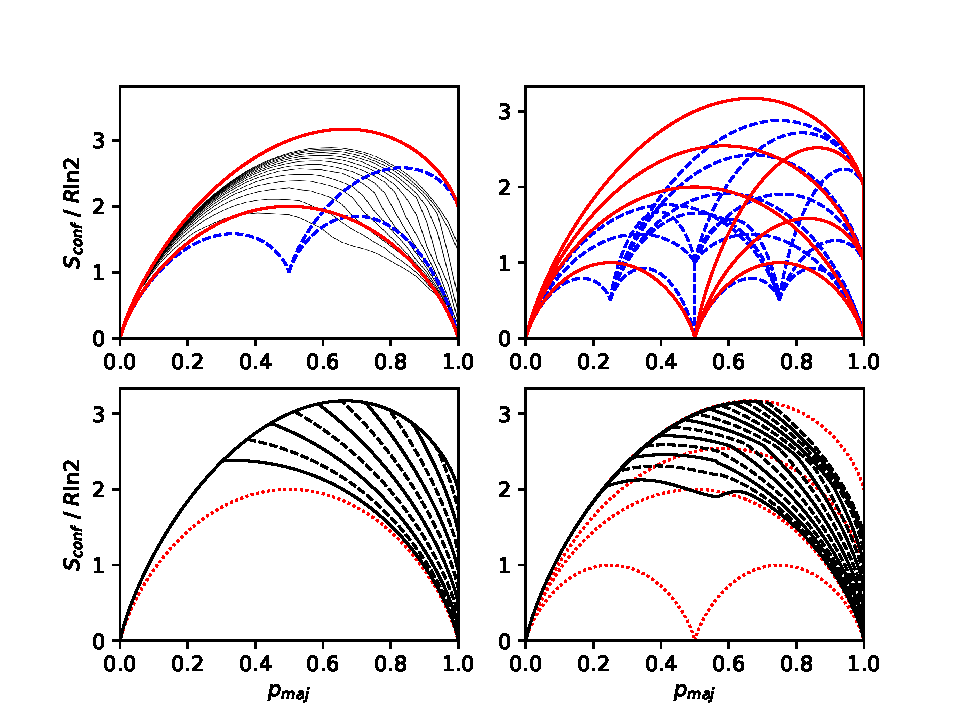
\includegraphics[width=\textwidth]{figures/py_maj_solution_entropies.pdf}
  \caption{Configurational entropy of two-site and four-site pyrope-majorite solution models. Entropies are calculated on a two-mole basis and nondimensionalised using the gas constant $R$. Top row: Independent endmember mixing in two-site (left) and four-site (right) pyrope-majorite. Grey dashed lines [?blue?] correspond to binary mixing lines between all endmembers; red solid lines to a subset of independent endmembers that guarantees continuous ordering with decreasing temperature (see Section \ref{sec:relative_stability}). The black lines in the top left panel are from an ab-initio study \citep{Vinograd2006}, with temperatures between 800$^{\circ}$C and 3400$^{\circ}$C. Bottom row: Example configurational entropies at equilibrium as a function of temperature, again between 800$^{\circ}$C and 3400$^{\circ}$C. Some of the endmember mixing lines from the upper panels are shown in red as guides. The two-site and four-site models both exhibit convergent ordering. In the four site model, the energy of Mg-Si mixing is doubled for two of the four sites. This simulates short-range Mg-Si order (see explanation in the main text). Model parameters are provided as supplementary materials.}
  \label{fig:pyrope_majorite_two_four_sites}
\end{figure}

\subsection{Identifying and avoiding ``logical inconsistencies" in solution models}
\label{sec:inconsistency}
If a solid solution model has fewer independent endmembers than that suggested by Equation \ref{eqn:site_mbr_relationship}, then the model includes at least one constraint which isn't related to charge-balance. Sometimes, these choices have been made consciously, with the aim of reducing the number of endmembers or to avoid dealing with order parameters. We have already met one example in Section \ref{sec:relative_stability}, where a partially disordered endmember in the two-site pyrope-majorite system (\ce{Mg3[Al][MgSi]Si3O12}) may be neglected if its energy and interaction energies are sufficiently high. However, there are many examples where reducing the number of independent endmembers is unreasonable. \citet{HP2006} used the example of Mg-Fe-Al orthopyroxene \ce{[Mg,Fe,Al][Mg,Fe](Al,Si)2O6} (where mixing on the tetrahedral site is not treated explicitly), and showed that splitting the Mg and Fe equally between the two sites resulted in a thermodynamically implausible solution.

Clinoamphibole provides a more complex example. One recent model includes 18 potential site-species, distributed over 6 sites \citep{Green2016,Holland2018}. A complete model in this system therefore has 12 independent endmembers. Table \ref{tab:camph_matrix} was computed using \emph{burnman} (see Appendix). The published model in this system has only 11 independent endmembers, but, unlike in the simple system, the inconsistency is not obvious. Equation \ref{eqn:site_mbr_relationship} is thus an extremely useful check for complex solution models. 


\begin{table}[htb!]
\centering
\scriptsize
\setlength{\tabcolsep}{4pt}
\begin{tabular}{l|lll|ll|lllll|llll|ll|ll}
               & \multicolumn{3}{l}{A (1)} & \multicolumn{2}{l}{M$_{13}$ (3)} & \multicolumn{5}{l}{M$_2$ (2)} & \multicolumn{4}{l}{M$_4$ (2)} & \multicolumn{2}{l}{T (4)} & \multicolumn{2}{l}{V (2)}   \\
name & v & Na & K & Mg & Fe & Mg & Fe & Al & Fe$^{3+}$ & Ti & Ca & Mg & Fe & Na & Si & Al & OH & O \\
\hline
tr & 1 & 0 & 0 & 1 & 0 & 1 & 0 & 0 & 0 & 0 & 1 & 0 & 0 & 0 & 1 & 0 & 1 & 0 \\
ts & 1 & 0 & 0 & 1 & 0 & 0 & 0 & 1 & 0 & 0 & 1 & 0 & 0 & 0 & 0.5 & 0.5 & 1 & 0 \\ 
parg & 0 & 1 & 0 & 1 & 0 & 0.5 & 0 & 0.5 & 0 & 0 & 1 & 0 & 0 & 0 & 0.5 & 0.5 & 1 & 0 \\ 
gl & 1 & 0 & 0 & 1 & 0 & 0 & 0 & 1 & 0 & 0 & 0 & 0 & 0 & 1 & 1 & 0 & 1 & 0 \\ 
cumm & 1 & 0 & 0 & 1 & 0 & 1 & 0 & 0 & 0 & 0 & 0 & 1 & 0 & 0 & 1 & 0 & 1 & 0 \\
grun & 1 & 0 & 0 & 0 & 1 & 0 & 1 & 0 & 0 & 0 & 0 & 0 & 1 & 0 & 1 & 0 & 1 & 0 \\
a & 1 & 0 & 0 & 1 & 0 & 0 & 1 & 0 & 0 & 0 & 0 & 0 & 1 & 0 & 1 & 0 & 1 & 0 \\ 
b & 1 & 0 & 0 & 0 & 1 & 1 & 0 & 0 & 0 & 0 & 0 & 0 & 1 & 0 & 1 & 0 & 1 & 0 \\ 
mrb & 1 & 0 & 0 & 1 & 0 & 0 & 0 & 0 & 1 & 0 & 0 & 0 & 0 & 1 & 1 & 0 & 1 & 0 \\ 
kprg & 0 & 0 & 1 & 1 & 0 & 0.5 & 0 & 0.5 & 0 & 0 & 1 & 0 & 0 & 0 & 0.5 & 0.5 & 1 & 0 \\
tts & 1 & 0 & 0 & 1 & 0 & 0 & 0 & 0 & 0 & 1 & 1 & 0 & 0 & 0 & 0.5 & 0.5 & 0 & 1 \\
famph & 1 & 0 & 0 & 0 & 1 & 0 & 0 & 1 & 0 & 0 & 0 & 0 & 1 & 0 & 1 & 0 & 0 & 1 
\end{tabular}
\caption{Independent endmember site-occupancy matrix $\boldsymbol{E}^{\textit{ind}}$ for a six-site clinoamphibole solution model including full order-disorder. Site multiplicities are given in brackets. The \emph{famph} endmember is one of many potential endmembers that completes the published endmember basis \citep{Green2016,Holland2018}. This solution model has a total of 432 endmembers.}
\label{tab:camph_matrix}
\end{table}

One may therefore ask how to determine whether any independent endmembers can be removed from a solution model. The following two points should be borne in mind:
\begin{itemize}
    \item Independent endmembers should not be removed if they exclude certain regions of chemical composition space from the solution model. 
    \item Endmembers which represent non-zero \textit{and} non-maximal entropies at their given composition \textit{may} be removed as long as they do not disobey the above rule, with the understanding that their removal will also render some of the full site-occupancy space inaccessible.
    \item Once a solution model has been constructed, it can be checked for regions of site-occupancy space and independent endmembers that never contribute to the lowest energy solution. This is what was done in Section \ref{sec:sro}, reducing the two-site model from four to three endmembers, and the four-site model from eight to five endmembers. 
\end{itemize}

\section{Manipulation of solid solution models}
\label{sec:manipulation}
\subsection{Changing independent endmember bases}
\label{sec:basis_conversion}

The previous section described how to consistently determine an independent endmember set for a solid solution, based on knowledge only of the set of distinct sites in the structure, and the potential species residing on each site. It also outlined potential pitfalls in attempts to simplify the resulting solution models. This section demonstrates how to convert between sets (or bases) of independent endmembers. This conversion has two primary purposes. Firstly, we often wish to solve thermodynamic problems in restricted compositional spaces. For example, we might want to model the almandine-skiagite binary in garnets (\ce{[Fe^{2+}]3[Fe^{3+},Al]2Si3O12}) using a solution model where almandine (\ce{[Fe^{2+}]3[Al]2Si3O12}), grossular (\ce{[Ca]3[Al]2Si3O12}) and andradite (\ce{[Ca]3[Fe^{3+}]2Si3O12}) are the independent endmembers. Secondly, we can use the same mathematics to solve the problem where we wish to convert atomic interactions (for example, the interaction between \ce{Fe^{2+}} on one site and \ce{Fe^{3+}} on another) into endmember interactions (for example, the interaction energy between almandine and andradite).


Throughout this section, the matrix $\boldsymbol{A}$ is used to transform an independent endmember basis to a new basis. Each element of $A_{ij}$ corresponds to the amount of original endmember $i$ contained within the new endmember $j$. The proportions of the original endmember set $p_i$ in terms of the new endmember set $p'_l$ are thus given by:
\begin{equation}
    p_i = A_{il}p'_l
\label{eqn:transform_proportions}
\end{equation}

The following subsections outline the mathematics to convert endmember bases within the ``ideal'', ``asymmetric'' and ``subregular'' mixing model formulations.

\subsubsection{The asymmetric model}
Changing endmember basis for the asymmetric model has been described in \citep{Diener2007}. It is included here both for completeness and to provide an alternative derivation using Einstein summation convention. The non-configurational Gibbs free energy is given by:
\begin{eqnarray}
    G^* &=& p_i G^{mbr}_i + \alpha_i p_i \alpha_j p_j W_{ij}^B/f \label{eqn:asymmetric_gibbs}\\
    f &=& \alpha_k p_k
\end{eqnarray}
where the components of $W_{ij}^B$ are equal to $2 W_{ij} / (\alpha_i + \alpha_j)$, and $\boldsymbol{W}$ is an upper triangular matrix containing the binary endmember interaction parameters. The endmember and interaction terms are computed separately. The endmember and interaction terms can be combined into a single combined matrix:
\begin{eqnarray}
    G^* &=& \alpha_i p_i \alpha_j p_j W^C_{ij} / f\\
    W^C_{ij} &=& W_{ij}^B + ((G^{mbr}/\alpha)_i 1_j + 1_i (G^{mbr}/\alpha)_j)/2 \label{eqn:asymmetric_combined}
\end{eqnarray} 
Substituting Equation \ref{eqn:transform_proportions} into this expression yields:
\begin{eqnarray}
    G^* &=& \alpha_i A_{il}p'_l \alpha_j A_{jm}p'_m W_{ij}^C/f \\
    f &=& \alpha_k A_{kn}p'_n 
    \label{eqn:asymmetric_t1}
\end{eqnarray}

In order to transform this new expression into the same form as Equation \ref{eqn:asymmetric_gibbs}, we first define new asymmetry parameters, and matrices $\boldsymbol{B}$ and $\boldsymbol{C}$:
\begin{eqnarray}
    \alpha'_l &=& \alpha_i A_{il}\\
    B_{il} \alpha'_l &=& C_{il} = \alpha_i A_{il}
\end{eqnarray} 
such that
\begin{equation}
    B_{il} = \alpha_i A_{il} (1/\alpha')_l
\end{equation}
Substituting these expressions into Equation \ref{eqn:asymmetric_t1} yields
\begin{eqnarray}
    G^* &=& B_{il} \alpha'_l p'_l B_{jm} \alpha'_m p'_m W_{ij}^C/f' \\
    f' &=& \alpha'_n p'_n 
    \label{eqn:asymmetric_t2}
\end{eqnarray}
The interaction matrix can now be transformed to yield an expression in the form of Equation \ref{eqn:asymmetric_gibbs}:
\begin{eqnarray}
    G^* &=& \alpha'_l p'_l \alpha'_m p'_m W'^C_{ij}/{f'}\\
    W'^C_{lm} &=& B_{il} B_{jm} W^C_{ij} 
\end{eqnarray}
The transformed endmember properties are now removed from the transformed binary. This is the reverse of the operation in Equation \ref{eqn:asymmetric_combined}:
\begin{eqnarray}
    G'^{mbr}_l &=& \alpha'_l W'^{C}_{ll} \\
    D_{lm} &=& W'^{C}_{lm} - \left((G'^{mbr}/\alpha')_l 1_m + 1_l (G'^{mbr}/\alpha')_m\right)/2
\end{eqnarray}
Finally, the binary can be converted back to upper triangular form by summing the upper and lower triangular components of $\boldsymbol{D}$:
\begin{equation}
    W'^B_{lm} = 
    \begin{cases}
        D_{lm} + D_{ml},& \text{if } l<m\\
        0,              & \text{otherwise}
    \end{cases}
\end{equation}
where the components of $W'^B_{lm}$ are equal to $2 W'_{lm} / (\alpha'_l + \alpha'_m)$.

\subsubsection{The subregular model}
%As far as I am able to tell, the basis transformation of the subregular model does not appear to have been published. 
In the subregular model, the non-configurational Gibbs free energy includes unary (endmember), binary and ternary contributions \citep{HW1989}:
\begin{equation}
    G^* = p_i G^{mbr}_i + p_i p_j W_{ij}^B (1 + p_j - p_i)/2 + p_i p_j p_k W_{ijk}^T
\end{equation}
where each of the three terms is computed separately. The superscript $T$ indicates that this is the ternary matrix, not the transpose [doesn't the ijk subscript suffice to indicate ternary tems?]. This equation can be transformed into a single term involving a combined interaction matrix $W^C$:
\begin{equation}
    G^* = p_i p_j p_k W^C_{ijk}
\end{equation}  
\begin{equation}
    \begin{split}
        W^C_{ijk} =& (G^{mbr}_i 1_j 1_k + G^{mbr}_j 1_i 1_k + G^{mbr}_k 1_i 1_j)/3 \\
        &+ (1_iW_{jk}^B + W_{ij}^B I_{jk} - W_{ij}^B I_{ik})/2 + W_{ijk}^T
    \end{split}
\end{equation}

Using the relationship between the original and transformed endmember proportions (Equation \ref{eqn:transform_proportions}):
\begin{equation}
    G^* = A_{il} p'_l A_{jm} p'_m A_{kn} p'_n W^C_{ijk}
\end{equation}
and so the transformed interaction matrix $W'^C$ is:
\begin{equation}
    W'^{C}_{lmn} = A_{il}A_{jm}A_{kn}W_{ijk}^C
\end{equation}
To convert this back into the original form, we first remove the transformed endmember excesses:
\begin{equation}
    G'^{mbr}_l = W'^{C}_{lll}
\end{equation}
\begin{equation}
    B_{lmn} = W'^{C}_{lmn} - (G'^{mbr}_l 1_m 1_n + 1_l G'^{mbr}_m 1_n + 1_l 1_m G'^{mbr}_n)/3
\end{equation}
The new binary matrix is then
\begin{equation}
    W'^B_{lm} = (B_{lmn} + B_{mln} + B_{mnl}) I_{mn}
\end{equation}
Removing this from the matrix leaves us with matrix $\boldsymbol{C}$:
\begin{equation}
    C_{lmn} = B_{lmn} - 1_l W'^B_{mn}/2
\end{equation}
The ternary components can then be found by summing the six contributing species of $\boldsymbol{C}$:
\begin{equation}
    W'^T_{lmn} = 
    \begin{cases}
        C_{lmn} + C_{mnl} + C_{nlm} + C_{nml} + C_{mln} + C_{lnm},& \text{if } l<m<n\\
        0,              & \text{otherwise}
    \end{cases}
\end{equation}

The lack of ternary terms in any particular multisite-solution endmember basis does not guarantee the lack of ternary terms in any other basis.

\subsection{Converting microscopic interactions into endmember interactions}
\label{sec:micro_to_macro}
The models presented so far are macroscopic models; they deal with the energetics of interaction between endmembers. Solution models can also be formulated in terms of atomic interactions. Microscopic models can be described by interaction matrices of the same form and dimension as their macroscopic counterparts, but the size of each dimension of the matrix is now equal to the number of site-species, rather than the number of endmembers. The elements of the matrix correspond to the site-species interactions. 

There are benefits to describing the properties of a solid solution in terms of microscopic interactions. Microscopic descriptions provide a much more direct link between the physics of the interactions (for example, order-disorder, Al-Al avoidance). In addition, \cite{Powell2014} argue that well-constrained values of microscopic interactions in one mineral can be used as informed guesses for other minerals. For example, Fe-Mg exchange interaction has a value of around 5 kJ per mole of sites in many silicate minerals. This concept, termed micro-$\phi$ [ref], may be useful for constructing complex models where there is insufficient data to fully constrain all interactions.

Despite the benefits of parameterising solutions using microscopic models, it is usually more practical to convert these to macroscopic models for computational purposes \citep{PH1993}. Macroscopic models require fewer parameters, automatically maintain charge balance, and the endmembers can be chosen to enable more efficient computations. The linear relationship between site-species proportions and endmember proportions (Equation \ref{eqn:proportions_to_sites}) has exactly the same form as the relationship between sets of independent endmembers (Equation \ref{eqn:transform_proportions}). Therefore, the conversion from a microscopic to a macroscopic formalism is simply another form of basis conversion, allowing the mathematics of Section \ref{sec:basis_conversion} to be used to convert from site interactions to endmember interactions. The untransformed endmember proportions $\boldsymbol{p}$ in Equation \ref{eqn:transform_proportions} are set equal to the site-species proportions $\boldsymbol{x}$, and the matrix $\boldsymbol{A} = \boldsymbol{E}^{\textit{ind}T}$. The endmember energies $\boldsymbol{G}'^{mbr}$ and (macroscopic) interaction matrices calculated using the equations of the previous section should be normalised to one mole of endmembers by multiplying them by $n_{\textrm{sites}}$.

The only remaining question is how to populate the microscopic interaction matrices. 

\subsubsection{Asymmetric model}
Binary microscopic interactions have two forms: simple mixing on a single site (e.g. \ce{Mg^{2+}} and \ce{Al^{3+}} on Site X), and combinations of species across sites (e.g. \ce{Mg^{2+}} on Site X and \ce{Ca^{2+}} on Site Y). Each entry in the matrix corresponds to an energy of formation of a cluster of sites $\epsilon_{[A]^X[C]^Y}$ from their constituents:
\begin{equation}
    \ce{[A]^X + [C]^Y -> [A]^X[C]^Y}
\end{equation}
For single-site mixing, the reaction can be rewritten as 
\begin{equation}
    \ce{[A]^X + [B]^X -> 2[A_{0.5}B_{0.5}]^X}
\end{equation}

If all upper-triangular (plus diagonal) components of the microscopic interaction matrix can be filled (with pressure-temperature-dependent energies), along with asymmetry parameters, then this is sufficient to obtain both the macroscopic interaction parameters and the endmember energies (again, P-T dependent). However, two-site energies ($\epsilon_{[A]^X[C]^Y}$) cannot be obtained from experimental analyses. Instead, the energies corresponding to cross-site reactions must be used. For example, the reaction
\begin{equation}
    \ce{[A]^X[C]^Y + [B]^X[D]^Y -> [B]^X[C]^Y + [A]^X[D]^Y}
\end{equation}
is associated with the cross-site interaction energy $w_{ACBD,XY}$, which is a function of the two-site energies (e.g. $\epsilon_{AB}$):
\begin{equation}
    w_{ACBD,XY} = (\epsilon_{BC} + \epsilon_{AD}) - (\epsilon_{AC} + \epsilon_{BD})
\end{equation}

For each two-site block of the microscopic interaction matrix, one element can be set to zero. Let us choose that element to be \ce{[B]^X[D]^Y}. All the remaining elements (\ce{[A]^X[C]^Y}) of that block are filled with values $-w_{ACBD,XY}$. Note that interaction energies $w_{BCBD,XY}$ and $w_{ADBD,XY}$ are always equal to zero \citep{PH1993}, because the corresponding reactions have the same products and reactants. 

A fully-worked example corresponding to that discussed in \cite{Powell2014} is included in the supplementary information.


\subsubsection{Subregular model}
The construction of the binary site interaction matrix for the subregular model $W^B_{ij}$ is much the same as for the asymmetric model, with the exception that the matrix is a full matrix, rather than an upper-triangular one. To construct the upper-triangular ternary matrix $W^T_{ijk}$, we start from the concept that each component of the matrix corresponds to an energy of formation of a cluster of sites $\epsilon_{[A]^X[C]^Y[E]^Z}$ from their constituents:
\begin{equation}
    \ce{[A]^X + [C]^Y + [E]^Z -> [A]^X[C]^Y[E]^Z}
\end{equation}
Mixing of three species on the same site can be rewritten:
\begin{equation}
    \ce{[A]^X + [C]^X + [E]^X -> 3[A_{\frac{1}{3}}C_{\frac{1}{3}}E_{\frac{1}{3}}]^X}
\end{equation}
For mixing of three species on two distinct sites, we have
\begin{equation}
    \ce{[A]^X + [C]^X + 2[E]^Y -> 2[A_{\frac{1}{2}}C_{\frac{1}{2}}]^X[E]^Y}
\end{equation}
The energy of formation of these three-element two-site complexes includes site-bonding terms which cannot be uniquely determined by experimental means. An example cross-site reaction would be
\begin{equation}
    \ce{[A_{0.5}C_{0.5}]^X[E]^Y + [B_{0.5}D_{0.5}]^X[E]^Y -> [B_{0.5}C_{0.5}]^X[E]^Y + [A_{0.5}D_{0.5}]^X[E]^Y}
\end{equation}
The number of independent components in the X-X-Y blocks of the ternary matrix will be $(m-1)^2(n)$, where $m$ and $n$ are the number of species on the X and Y sites. Finally, for a three-site exchange, the cross site reactions will be of the form:
\begin{equation}
\begin{split}
    \ce{[A]^X[C]^Y[E]^Z + [B]^X[D]^Y[E]^Z + [B]^X[C]^Y[F]^Z + [A]^X[D]^Y[F]^Z -> \\
    [B]^X[D]^Y[F]^Z + [A]^X[C]^Y[F]^Z + [A]^X[D]^Y[E]^Z + [B]^X[C]^Y[E]^Z}
\end{split}
\end{equation}
The number of independent components in the X-Y-Z blocks of the ternary matrix will be $(m-1)(n-1)(o-1)$, where $m$, $n$ and $o$ are the number of species on the X, Y and Z sites.

\section{Discussion}
\label{sec:discussion}

\subsection{Using the microscopic formulation}
%\subsubsection{Complexity of the microscopic formulation}
%\subsubsection{On the use of heuristics}

\subsubsection{Convergent ordering and the microscopic formulation}

If similar interactions in the microscopic interaction matrix $\mathbf{w}$ are taken to be equal to each other, and if the energies of the ordered endmembers relative to the disordered endmembers in the solid solution are derived from the conversion described in Section \ref{sec:manipulation}, the resulting model is guaranteed to exhibit globally convergent ordering (i.e. the system will become completely disordered at a composition-dependent critical temperature). 


\subsubsection{Automated site splitting}

Using the microscopic formulation also allows the user to arbitrarily continue splitting sites, without necessarily increasing the number of independent parameters. This can serve two purposes. Firstly, it provides a potentially easy way to match ordering observed at intermediate compositions (as demonstrated for the pyrope-majorite system in Section \ref{sec:sro}). Secondly, it potentially serves as a useful check on the parameters chosen in a simpler model. If a split-site model results in an unrealistically stable ordered compound, the microscopic interactions can be modified to better fit the observations.

% For example, take the two-site majorite solution given in Table \ref{tab:maj2_polytope}. In a regular/symmetric solution model, this solution requires ten independent non-zero interaction energies (not including the six self-energies of the site-species): w(AlMg,Y1), w(AlSi,Y1), w(MgSi,Y1), w(AlMg,Y2), w(AlSi,Y2), w(MgSi,Y2), w(MgMgAlAl,Y1Y2), w(MgSiAlAl,Y1Y2), w(SiMgAlAl,Y1Y2) and w(SiSiAlAl,Y1Y2). If the sites are treated as identical, then only six of these ten are distinct (because w(AlMg,Y1)=w(AlMg,Y2), w(AlSi,Y1)=w(AlSi,Y2), w(MgSi,Y1)=w(MgSi,Y2) and w(MgSiAlAl,Y1Y2)=w(SiMgAlAl,Y1Y2)). Whatever the values chosen for these six interaction energies, the resulting endmember energies and interaction energies will result in convergent ordering. 

\subsection{Checking site-occupancy space for globally unstable/metastable regions}
\textcolor{red}{Is this something we can do without resorting to brute force? The PerpleX pseudocompound method is actually pretty powerful in this respect (and would work for any solution model), but I wonder whether there's a way in which we can exploit endmember activities or their derivatives.}

\section{Concluding remarks}




\appendix
\section{\emph{burnman} implementations}
Users of the software package \emph{burnman} can calculate all the possible endmember site occupancies of a solid solution, and an independent subset of those endmembers using the functions
\begin{verbatim}
feasible_endmember_occupancies_from_charge_balance()
independent_endmember_occupancies_from_charge_balance()
\end{verbatim}
both of which are contained in the solidsolution module. 

The set of feasible dependent endmembers of any solution model can be found using the function
 \begin{verbatim}
 dependent_endmember_site_occupancies()
 \end{verbatim}
which is again contained in the solidsolution module. 

Conversions from microscopic to macroscopic interaction parameters can be computed both in symbolic form (through python's \emph{sympy} module) and in numeric form using \emph{burnman}'s \emph{microphi} module. 

See the supplementary file for examples and output. 

% Other stuff on polytopes online
% porta http://porta.zib.de/, also polymake http://www.math.tu-berlin.de/polymake/
% FAQ pdf from Fukuda









%% The Appendices part is started with the command \appendix;
%% appendix sections are then done as normal sections
%% \appendix

%% \section{}
%% \label{}

%% References
%%
%% Following citation commands can be used in the body text:
%% Usage of \cite is as follows:
%%   \cite{key}          ==>>  [#]
%%   \cite[chap. 2]{key} ==>>  [#, chap. 2]
%%   \citet{key}         ==>>  Author [#]

%% References with bibTeX database:

\bibliographystyle{model1-num-names}
\bibliography{references.bib}

%% Authors are advised to submit their bibtex database files. They are
%% requested to list a bibtex style file in the manuscript if they do
%% not want to use model1-num-names.bst.

%% References without bibTeX database:

% \begin{thebibliography}{00}

%% \bibitem must have the following form:
%%   \bibitem{key}...
%%

% \bibitem{}

% \end{thebibliography}


\end{document}

%%
%% End of file `elsarticle-template-1-num.tex'.